\input{../../../stock/en-tete_v6.tex}

\newcommand{\titrechapitre}{Fonctions exponentielle et logarithme népérien}
\newcommand{\numerochapitre}{1}

\renewcommand{\headrulewidth}{0.4pt}
\renewcommand{\footrulewidth}{0.4pt}
\fancyfoot[L]{Raphaël JONTEF}
\fancyfoot[C]{\thepage}
\fancyfoot[R]{\href{https://www.alveusclub.com/}{Alveus}}
\fancyhead[L]{Mathématiques : Terminale}
\fancyhead[R]{\titrechapitre}

\begin{document}
\input{../../../stock/commands.tex}

% Page de titre custom
\setlength{\headheight}{15pt}
\begin{titlepage}
    \centering
    \vspace*{3cm}
    {\huge Chapitre \numerochapitre\par}
    {\Huge \bfseries\titrechapitre\par}
    \vspace{8cm}
    {\Large Cours rédigé par Raphaël JONTEF\par}
    \vspace{2em}
    {\small \textit{raphaeljontef@hotmail.com}\par}
    \vspace{2cm}

    {\normalsize pour un enseignement dans le cadre  \par}
    {\small d'un soutien scolaire encadré par \href{https://www.alveusclub.com/}{Alveus} \par}
    \vfill
    {\large \today\par}
\end{titlepage}


\section{Fonction exponentielle}
\subsection{Définition, notation}

\begin{definition}{}{fonction exponentielle}
    La \notion{fonction exponentielle} est l'unique fonction $f$ égale à sa dérivée, prenant la valeur $1$ en $0$. On la note $\exp$~:
    \fonction{\exp}{\R}{\R_+}{x}{e^x}
    où $e \approx 2,71828$ est le nombre d'Euler, c'est un nombre irrationnel.
\end{definition}

\begin{remarque}{}{}
    On a $e = e^1 = \exp(1)$.
\end{remarque}

\begin{figure}[ht]
    \centering
    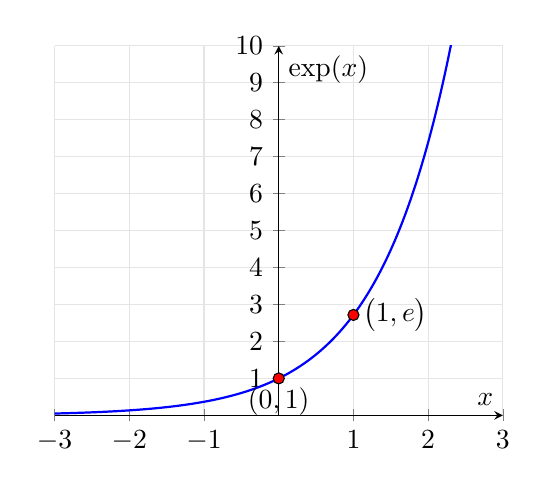
\begin{tikzpicture}
        \begin{axis}[
            width=0.6\textwidth,
            ymin=0, ymax=10,
            xmin=-3, xmax=3,
            xlabel=$x$, ylabel=$\exp(x)$,
            axis lines=middle,
            samples=200,
            domain=-3:3,
            grid=both,
            grid style={gray!20},
            xtick={-3,-2,-1,0,1,2,3},
            ytick={0,1,2,3,4,5,6,7,8,9,10},
            clip=true,
        ]
            \addplot[blue, thick] {exp(x)};
            % Points remarquables
            \addplot[only marks, mark=*, mark options={fill=red}] coordinates {(0,1) (1,2.71828)};
            \node[anchor=north] at (axis cs:0,1) {$(0,1)$};
            \node[anchor=west] at (axis cs:1,2.71828) {$\big(1,e\big)$};
        \end{axis}
    \end{tikzpicture}
    \caption{Graphe de $\exp$ sur $[-3,3]$.}
\end{figure}

\subsection{Propriétés de la fonction exponentielle}

\begin{theoreme}{}{propriété fondamentale de l'exponentielle}
    Pour tous réels $a$ et $b$, on a~:
    $$e^{a+b} = e^a \times e^b$$
\end{theoreme}

\begin{proposition}{}{découlant de la propriété fondamentale de l'exponentielle}
    \begin{enumeratebf}
        \item $e^{a-b} = \frac{e^a}{e^b}$
        \item $e^{na} = (e^a)^n$ pour tout $n \in \Z$
    \end{enumeratebf}
\end{proposition}

\begin{proposition}{}{invariance par dérivation}
    La fonction exponentielle est dérivable sur $\R$ et pour tout $x \in \R$~:
    $$\big(e^x\big)' = e^x$$
    La fonction exponentielle est donc strictement croissante sur $\R$.
\end{proposition}

\begin{proposition}{}{dérivée de $\exp(u)$}
    Si $u$ est une fonction dérivable sur un intervalle $I$, alors la fonction $\exp\Big(u(x)\Big)$ est dérivable sur $I$ et pour tout $x \in I$~:
    $$\big(e^{u(x)}\big)' = u'(x) \times e^{u(x)}$$
\end{proposition}

\subsection{Approfondissement, limites de l'exponentielle}

\begin{proposition}{}{limites de l'exponentielle}
    On a~:
    \begin{itemize}
        \item $\displaystyle \lim_{x \to -\infty} e^x = 0$
        \item $\displaystyle \lim_{x \to +\infty} e^x = +\infty$
    \end{itemize}

\end{proposition}

\begin{theoreme}{}{de croissances comparées}
    Pour tout $n \in \N^*$, on a~:
    $$\lim_{x \to +\infty} \frac{e^x}{x^n} = +\infty$$
\end{theoreme}

\begin{remarque}{}{}
    En utilisant ce théorème, on intègrera la mention "Par croissances comparées".
\end{remarque}  




\section{Fonction logarithme népérien}
\subsection{Définition, notation}
\begin{definition}{}{fonction logarithme népérien}
    La \notion{fonction logarithme népérien} est la fonction réciproque de la fonction exponentielle. On la note $\ln$~:
    \fonction{\ln}{\R_+^*}{\R}{x}{\ln(x)}
\end{definition}

\begin{definition}{}{officielle du programme de terminale Générale}
    En terminale générale, on définit la fonction logarithme népérien $\ln$ comme l'unique primitive de $x \to \frac{1}{x}$, s'annulant en $1$.\\
    En effet, $\ln$ est dérivable sur $\R_+^*$ et $\ln': x \mapsto \frac{1}{x}$.
\end{definition}

\begin{remarque}{}{}
    Puisque $\ln$ est la fonction réciproque de $\exp$, on a pour tout $x \in \R_+^*$~:
    $$\ln(e^x) = x \quad \text{et} \quad e^{\ln(x)} = x$$
\end{remarque}

% Plot de la fonction ln sur un domaine significatif
\begin{figure}[ht]
    \centering
    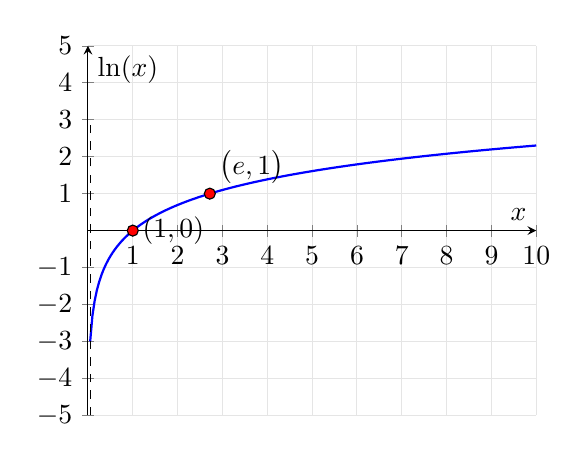
\begin{tikzpicture}
        \begin{axis}[
            width=0.6\textwidth,
            xmin=0, xmax=10,
            ymin=-5, ymax=5,
            xlabel=$x$, ylabel=$\ln(x)$,
            axis lines=middle,
            samples=200,
            domain=0.05:10,
            grid=both,
            grid style={gray!20},
            ytick={-5,-4,-3,-2,-1,0,1,2,3,4,5},
            xtick={0,1,2,3,4,5,6,7,8,9,10},
            clip=false,
        ]
            \addplot[blue, thick] {ln(x)};
            % Points remarquables
            \addplot[only marks, mark=*, mark options={fill=red}] coordinates {(1,0) (2.71828,1)};
            \node[anchor=west] at (axis cs:1,0) {$(1,0)$};
            \node[anchor=south west] at (axis cs:2.71828,1) {$\big(e,1\big)$};
            % Asymptote visuelle près de 0
            \draw[dashed] (axis cs:0.05,-5) -- (axis cs:0.05,3);
        \end{axis}
    \end{tikzpicture}
    \caption{Graphe de $\ln$ sur $[0.05,10]$.}
\end{figure}


\subsection{Propriétés du logarithme népérien}

\begin{theoreme}{}{propriété fondamentale du logarithme}
    Pour tous réels strictement positifs $a$ et $b$, on a~:
    $$\ln(ab) = \ln(a) + \ln(b)$$
\end{theoreme}

\begin{proposition}{}{découlant de la propriété fondamentale du logarithme}
    \begin{enumeratebf}
    \item $\ln(a/b) = \ln(a) - \ln(b)$
    \item $\ln(a^n) = n \ln(a)$ pour tout $n \in \Z$
    \end{enumeratebf}
\end{proposition}

\begin{proposition}{}{dérivée de $\ln(u)$}
    Si $u$ est une fonction dérivable et strictement positive sur un intervalle $I$, alors la fonction $\ln\Big(u(x)\Big)$ est dérivable sur $I$ et pour tout $x \in I$~:
    $$\big(\ln\Big(u(x)\Big)\big)' = \frac{u'(x)}{u(x)}$$
    $\ln$ est donc strictement croissante sur son domaine de définition.
\end{proposition}

\subsection{Approfondissement, limites de $\ln$}

\begin{proposition}{}{limites de $\ln$}
    On a~:
    \begin{itemize}
        \item $\displaystyle \lim_{x \to 0^+} \ln(x) = -\infty$
        \item $\displaystyle \lim_{x \to +\infty} \ln(x) = +\infty$
    \end{itemize}

\end{proposition}

\begin{theoreme}{}{de croissances comparées}
    Pour tout $n \in \N^*$, on a~:
    $$\lim_{x \to +\infty} \frac{\ln(x)}{x^n} = 0$$
\end{theoreme}

\begin{remarque}{}{}
    En utilisant ce théorème, on intègrera la mention "Par croissances comparées".
\end{remarque}





\end{document}